\documentclass{beamer}

\usepackage{tikz}

\newcommand{\myArrow}{-{Latex[length=3mm, width=2mm]}}

\begin{document}

\begin{frame}
	\begin{center}
		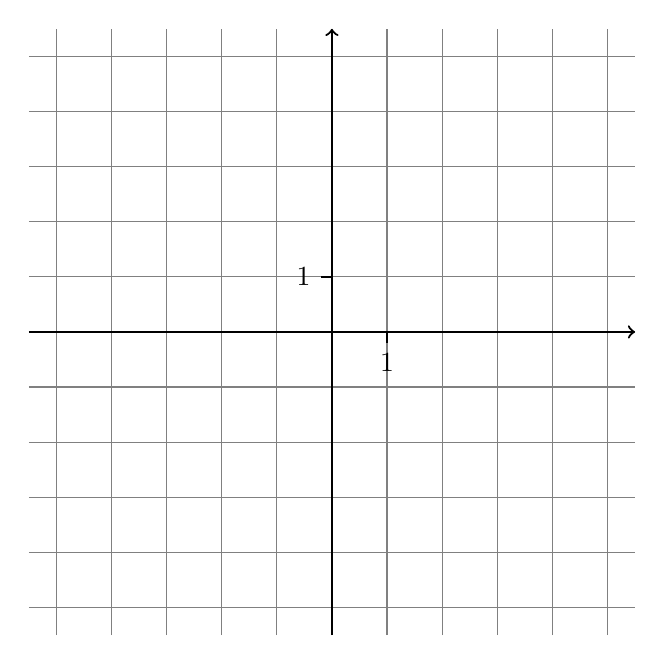
\begin{tikzpicture}[scale=0.7]
			\draw[thin,gray] (-5.5,-5.5) grid (5.5,5.5);
			\draw[thick,->] (-5.5,0) -- (5.5,0);
			\draw[thick,->] (0,-5.5) -- (0,5.5);
			\draw[thick] (1,0) -- ++(0,-0.2) node[below] {$1$}; 
			\draw[thick] (0,1) -- ++(-0.2,0) node[left] {$1$}; 
		\end{tikzpicture}
	\end{center}
\end{frame}

\end{document}